\documentclass[margin=5pt]{standalone}

\usepackage{tikz}
\usetikzlibrary{positioning,automata, matrix, trees}
\usetikzlibrary{calc,backgrounds}
\usetikzlibrary{arrows}
\usetikzlibrary{patterns,snakes}
\usepackage[default]{opensans}
\usepackage{tudscrcolor}
\usepackage{sfmath}
\begin{document}
%	\sffamily
	\color{cddarkblue}
	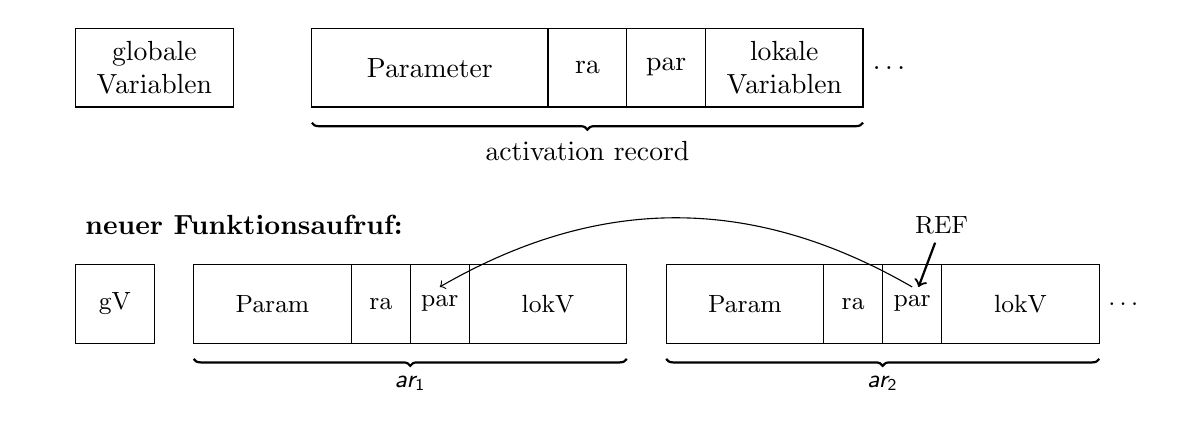
\begin{tikzpicture}[scale=1]
		\draw[] (0,0) rectangle ++(2,1) node[pos=.5, align=center, text width=2cm] (gv) {globale Variablen};
		
		\draw[] (3,0) rectangle ++(3,1) node[pos=.5, align=center, text width=3cm] (param) {Parameter};
		\draw[] (6,0) rectangle ++(1,1) node[pos=.5, align=center, text width=1cm] (ra) {ra};
		\draw[] (7,0) rectangle ++(1,1) node[pos=.5, align=center, text width=1cm] (par) {par};
		\draw[] (8,0) rectangle ++(2,1) node[pos=.5, align=center, text width=2cm] (lv) {lokale Variablen};
		\node[anchor=west] at (10,.5) {\dots};
		
		\draw [thick,
		decoration={
			brace,
			mirror,
			raise=0.2cm
		},
		decorate
		] (3,0) -- (10,0) 
		node [pos=0.5,anchor=north,yshift=-0.3cm] {activation record};
		
		\node[anchor=west] at (0,-1.5) {\textbf{neuer Funktionsaufruf:}};
		
		\small
		
		\draw[] (0,-3) rectangle ++(1,1) node[pos=.5, align=center, text width=2cm] (gv2) {gV};
		
		\draw[] (1.5,-3) rectangle ++(2,1) node[pos=.5, align=center, text width=3cm] (param2) {Param};
		\draw[] (3.5,-3) rectangle ++(.75,1) node[pos=.5, align=center, text width=1cm] (ra2) {ra};
		\draw[] (4.25,-3) rectangle ++(.75,1) node[pos=.5, align=center, text width=1cm] (par2) {par};
		\draw[] (5,-3) rectangle ++(2,1) node[pos=.5, align=center, text width=2cm] (lv2) {lokV};
		
		\draw[] (7.5,-3) rectangle ++(2,1) node[pos=.5, align=center, text width=3cm] (param2b) {Param};
		\draw[] (9.5,-3) rectangle ++(.75,1) node[pos=.5, align=center, text width=1cm] (ra2b) {ra};
		\draw[] (10.25,-3) rectangle ++(.75,1) node[pos=.5, align=center, text width=1cm] (par2b) {par};
		\draw[] (11,-3) rectangle ++(2,1) node[pos=.5, align=center, text width=2cm] (lv2b) {lokV};
		\node[anchor=west] at (13,-2.5) {\dots};
		
		\path[->, bend right] (par2b.north) edge (par2.north);
		\node (ref) at (11,-1.5) {REF};
		\draw[->, thick] (ref) -- (par2b);
		
		
		\draw [thick,
		decoration={
			brace,
			mirror,
			raise=0.2cm
		},
		decorate
		] (1.5,-3) -- (7,-3) 
		node [pos=0.5,anchor=north,yshift=-0.3cm] {$ar_1$};
		
		\draw [thick,
		decoration={
			brace,
			mirror,
			raise=0.2cm
		},
		decorate
		] (7.5,-3) -- (13,-3) 
		node [pos=0.5,anchor=north,yshift=-0.3cm] {$ar_2$};
	\end{tikzpicture}
\end{document}